% !TeX spellcheck = en_US
%\setcounter{chapter}{6} % set chapter counter so we begin at chapter 5
%\chapter{Laboration: PI/PID control of The Classroom Exo}


\section{Lab Introduction}

\begin{tcolorbox}[colback=blue!5!white,colframe=blue!75!black,title=Summary]
	In this chapter you will find the necessary documentation to setup your Classroom Exo, and try out the PI and PID controller options. We have prepared some Lab exercises, to help you learn more about control theory.
\end{tcolorbox}
\vspace{0.5cm}
 
An exoskeleton is a wearable mechanical structure that enhances or restores the physical abilities of the wearer by providing external support or amplification of movements \cite{AlTashi2024}. As the field of robotics grows leaps and bounds with every passing day as the world of STEM aims to integrate technology with humans to aid and support or enhance activities of daily living. Education leveraging these technologies has however been lacking. 
This lab is intended for use at a university level and is a derivative of a project aimed at converting an open-source exoskeleton into educational material \cite{AlTashi2024}. The Classroom Exo, the product that we will be using through the course of this lab, is a student-friendly optimized version of the EduExo Pro - An Advanced Robotic Exoskeleton Kit developed by Auxivo AG. 

\subsection{Risk section}
The Classroom Exo is not categorized as a medical device. Instead, its primary focus is educational. It is designed to provide hands-on experience with various control systems. There are some risks associated with the use of the Classroom Exo. Listed below are the potential risks, what has been done to prevent them, and the possible causes of these risks.
\begin{itemize}[]
	\item Muscle fatigue: Muscle fatigue can occur during prolonged use, as the Classroom Exo is somewhat heavy. To minimize this risk, an ergonomic design and proper usage guidelines have been implemented.
	\item Injury risk: The risk of injury is very low, but it still exists. The primary cause is misalignment between the Classroom Exo's mechanical joints and the user's shoulder and elbow joints. This risk has been minimized through proper calibration, an emergency stop feature, and clear instructions for how to put on the Classroom Exo.
\end{itemize}
	
\subsection{Learning objectives}
The goal of this section is to explore various step signals, plant designs, and control parameter settings to observe their effect on overshoot, oscillations, and residual error on step responses. You will reflect on the importance of control system design in biomedical applications where precise control is important for user safety.

\begin{itemize}[]
	\item Identify a PID controller's components and explain their effect on a system’s behavior.
	\item 	Demonstrate tuning of PID control and design parameters, predict and analyze their impact on system performance such as overshoot, oscillation and error.
	\item Evaluate the importance of the PI/PID controller in biomedical applications, specifically as applied to exoskeletons.
\end{itemize}
	
\subsection{Prerequisite knowledge}
For this section of the lab the students are expected to have a basic understanding of control systems, specifically P, PI and PID-controllers, the impact of each component in a PID controller and knowledge of the design and control parameters stated in the book “Fundamentals of Control Technology” \cite{Lennartson2002} . The students should be familiar with concepts like overshoot, oscillations and steady-state error. For example would this lab fit well in an engineering programme in the first control system course after introducing PID controllers. 

\subsection{Materials and methods}
For this lab, you will need a Bluetooth-enabled computer and MATLAB 2023b (although newer versions should also work). We will be interfacing with the exoskeletons using the “Updated BT-GUI” MATLAB application. Additionally, you will need one exoskeleton and a screwdriver to adjust the arm length of the exoskeleton to fit the anatomy of the student who will be wearing the exoskeleton.

\subsection{To do at home before the lab}
To make the most of the limited time you will have with the exoskeletons, you must come to the lab session well-prepared. Unforeseen issues or complications with the setup of the exoskeletons may arise, so proper preparation will ensure you have as much hands-on time as possible with the exoskeleton. Therefore before the lab asks you to: 
\begin{enumerate}[]
	\item Download MATLAB 2023b.
	\item Download the “Updated BT-GUI\_10-24”  folder from the GitHub link: \url{https://github.com/fabianjust/classroom-exo}
	\item Download and install the following MATLAB packages: 
	\begin{itemize}[]
		\item Control System Toolbox (version 23.2)
		\item Instrument Control Toolbox (version 23.2)
		\item Robotics System Toolbox (version 23.2)
		\item Sensor Fusion and Tracking Toolbox (version 23.2)
		\item Signal Processing Toolbox (version 23.2)
		\item Symbolic Math Toolbox (version 23.2)
	\end{itemize}
	\item Read the lab PM thoroughly.
\end{enumerate}


\newpage
	
\section{Introduction to the Exoskeleton}
Exoskeletons are increasingly being incorporated into rehabilitative settings, such as walking assists for people who have undergone spinal cord injuries, strokes, etc., in physiotherapy, and occupational therapy \cite{Hill2017}. Although aimed to be used in educational settings only, the Classroom Exo is an exoskeleton connected to the upper part of the body, over the shoulder, and the upper and lower arm, with a spring support to help lift the arm \autoref{fig:fig02}. Programmed on Arduino, it has three control systems - proportional–integral–-derivative controller (PID Controller), Electromyography signals from the muscles, and a force sensor on the wrist, the software of which is accessible as open-source, with a classroom-friendly graphical interface implemented on MATLAB. 

\begin{figure}[H]
	\centering
	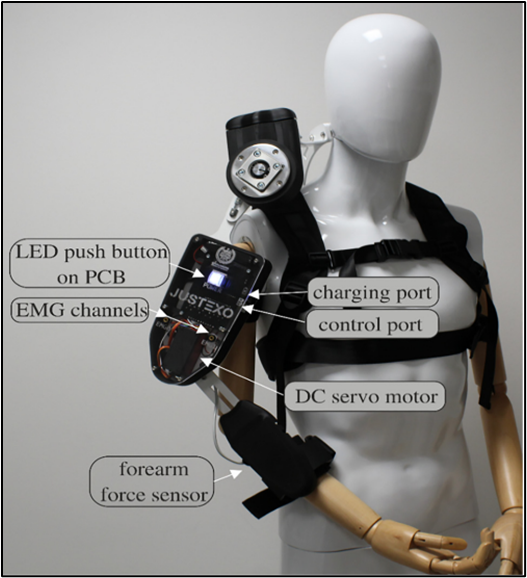
\includegraphics[width=0.7\linewidth]{img/fig_02}
	\caption{The Classroom Exo and its adaptations from EduExo Pro }
	\label{fig:fig02}
\end{figure}

\subsection{Setting up the Classroom Exo}
While putting on the exoskeleton it is helpful if one person holds it up and another tightens the straps.
\begin{enumerate}[]
	\item Put on the vest and fasten the buckles. 
	\item Make sure that the shoulder part of the exoskeleton is aligned with your shoulder, which can be seen in \autoref{fig:fig03}. And then tighten the chest and waist straps.
\end{enumerate}

\begin{figure}[H]
	\centering
	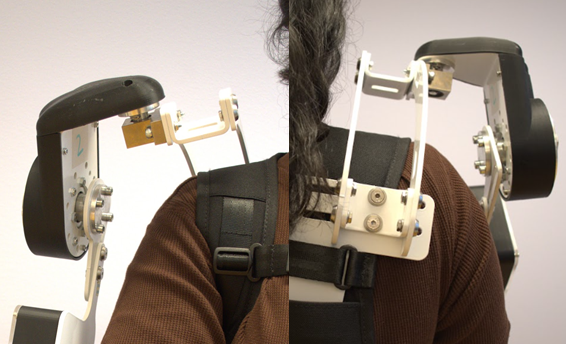
\includegraphics[width=0.4\linewidth]{img/fig_03}
	\caption{Shoulder joint aligned (left) and misaligned (right).}
	\label{fig:fig03}
\end{figure}

\begin{enumerate}[]
	\setcounter{enumi}{2}
	\item Tighten the straps around the elbow and the wrist and check alignment with the elbow joint according to \autoref{fig:fig04}. 
\end{enumerate}

\begin{figure}[H]
	\centering
	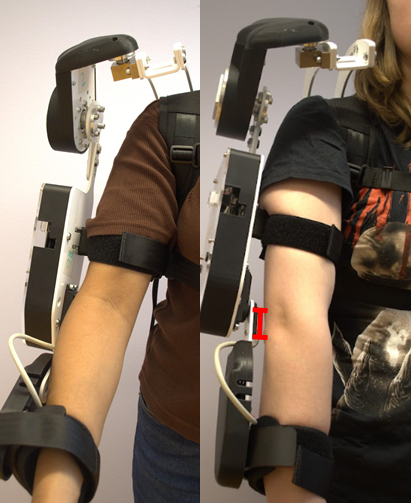
\includegraphics[width=0.4\linewidth]{img/fig_04}
	\caption{Correct alignment of elbow joint (left) and incorrect alignment (right), misalignment marked in red.}
	\label{fig:fig04}
\end{figure}

\begin{enumerate}[]
	\setcounter{enumi}{3}
	\item If the Classroom Exo has the correct joint alignment as seen in figure 4 and 3, proceed to section 2.1.2. If not, proceed with section 2.1.1 “Adjusting the exoskeleton”.
\end{enumerate}

\subsubsection{Adjusting the exoskeleton}
To be able to adjust the arm length of the Classroom Exo, a 2.5 and 3.0 Allen Key is needed.

\begin{enumerate}[]
	\item Under the shoulder joint on the back of the exoskeleton you can find two bolts for which the 3.0 Allen Key fits, the bolts are marked in \autoref{fig:fig05}. Loosen these, align shoulder joints according to \autoref{fig:fig03} and tighten the bolts. 
\end{enumerate}



\begin{figure}[H]
	\centering
	\begin{center}
		\begin{tikzpicture}
			\node(a){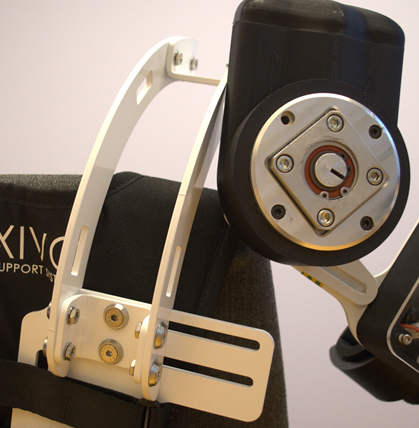
\includegraphics[width=0.4\linewidth]{img/fig_05}};
			\node at(a.center)[draw, red,line width=3pt,circle, minimum width=45pt, minimum height=45pt,rotate=-40,yshift=-65pt]{};
		\end{tikzpicture}   
	\end{center}
	\caption{Bolts for adjusting shoulder breadth in red.}
	\label{fig:fig05}
\end{figure}



\begin{enumerate}[]
	\setcounter{enumi}{1}
	\item To align the elbow, loosen the bolts on the inside of the shoulder joint illustrated in \autoref{fig:fig06}. Use the 3.0 Allen key to do this. Slide the arm such that the elbow joint of the exoskeleton and the user is aligned such as in \autoref{fig:fig04}. Tighten the bolts.
\end{enumerate}

\begin{figure}[H]
	\centering
	\begin{center}
		\begin{tikzpicture}
			\node(a){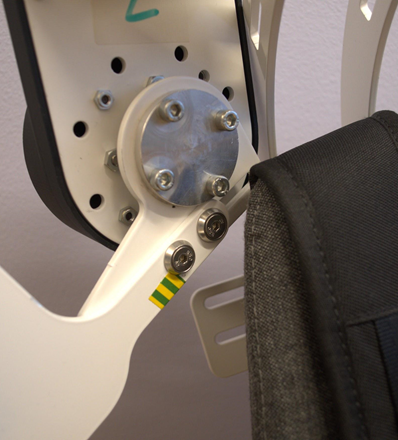
\includegraphics[width=0.4\linewidth]{img/fig_06}};
			\node at(a.center)[draw, red,line width=3pt,circle, minimum width=45pt, minimum height=45pt,rotate=0,yshift=-7pt, xshift=-1pt]{};
		\end{tikzpicture}   
	\end{center}
	\caption{Bolts to adjust upper arm length for elbow alignment marked in red.}
	\label{fig:fig06}
\end{figure}



\begin{enumerate}[]
	\setcounter{enumi}{2}
	\item To adjust the position of the wrist cuff, loosen the bolt on the lower part on the arm of the exoskeleton marked in \autoref{fig:fig07}, using the 2.5 Allen key. Adjust length and tighten the bolts.
\end{enumerate} 

\begin{figure}[H]
	\centering
	\begin{center}
		\begin{tikzpicture}
			\node(a){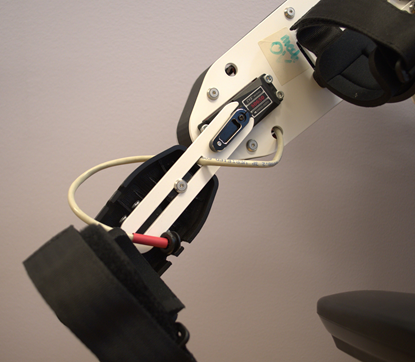
\includegraphics[width=0.4\linewidth]{img/fig_07}};
			\node at(a.center)[draw, red,line width=3pt,circle, minimum width=15pt, minimum height=15pt,rotate=0,xshift=-12pt, yshift=-2pt]{};
		\end{tikzpicture}   
	\end{center}
	\caption{Bolts to adjust lower arm length for positioning of wrist cuff marked in red.}
	\label{fig:fig07}
\end{figure}
\subsubsection{Connecting to the device and starting the GUI}
\begin{enumerate}[]
	\item Turn on the exoskeleton by pushing the “LED push button on PCB” as seen in \autoref{fig:fig08}. It  should blink blue indicating that it is searching for a Bluetooth device.
	\item When you are connecting to the exoskeleton for the first time, go to your computer's Bluetooth settings and add a Bluetooth device. When pairing, the name of your device will be XX\_CLASSROOM\_EDU\_EXO\_PRO where the XX is a number between 01 to 08 depending on which exoskeleton you have.
\end{enumerate}

\begin{figure}[H]
	\centering
	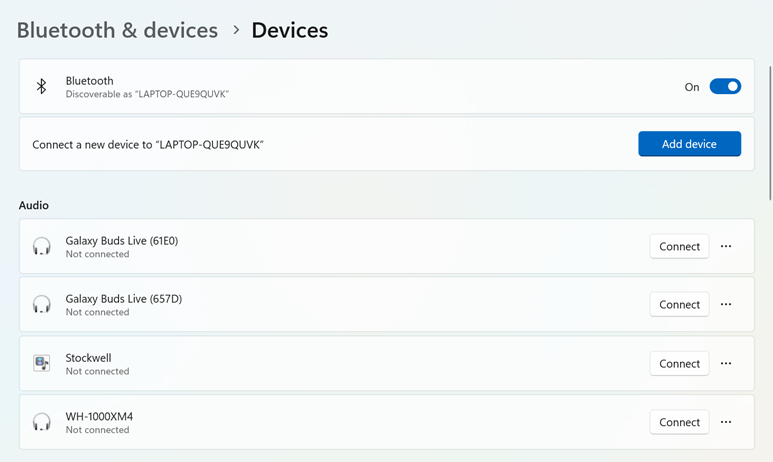
\includegraphics[width=0.7\linewidth]{img/fig_08}
	\caption{Pairing to a Bluetooth device for the first time.}
	\label{fig:fig08}
\end{figure}
\begin{enumerate}[]
	\setcounter{enumi}{2}
	\item In your computer's display settings set the screen size to 100\%.
\end{enumerate}
\begin{figure}[H]
	\centering
	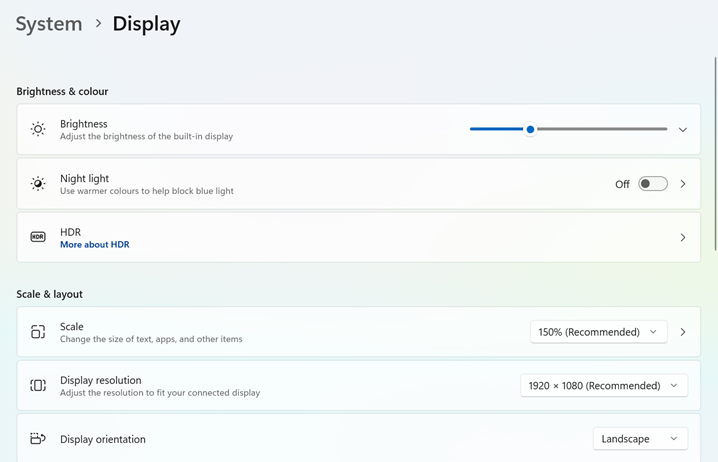
\includegraphics[width=0.7\linewidth]{img/fig_09}
	\caption{Changing screen sizing.}
	\label{fig:fig09}
\end{figure}

\begin{enumerate}[]
	\setcounter{enumi}{3}
	\item Open MATLAB, locate the BT\_GUI file and double click on it. Or locate the file in your file explorer and select open with MATLAB. If you open the file in MATLAB’s app designer, click run.
	\item When the GUI is opened, choose the correct Bluetooth device, and click connect. 
\end{enumerate}

\begin{figure}[H]
	\centering
	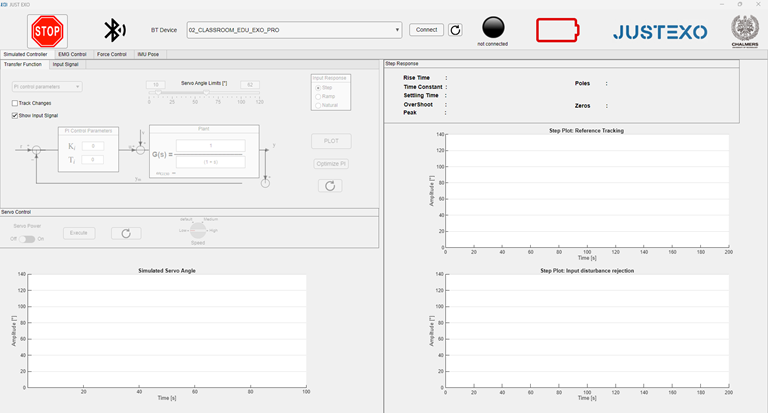
\includegraphics[width=0.7\linewidth]{img/fig_10}
	\caption{Connecting to the Bluetooth device.}
	\label{fig:fig10}
\end{figure}

The power button on the exoskeleton and the indicator in the GUI should change color to either green, yellow or red depending on the battery level.


\newpage
\section{PI/PID controller}
Introduction
The Classroom Exos’ software is capable of simulating two types of control systems: a PI controller and a PID controller. In total, six controllers are pre-installed. The first four are based on Bengt Lennartson's theories from his book “Fundamentals of Control Technology”[2], while the remaining two are standard PI/PID controllers. 

The PI controller consists of a proportional P action and an integrating I action. The PID controller also has a derivative D action. The design parameters that can be changed in the simulation for the PI controller are the upper crossover frequency ($\omega_c$) and the phase margin ($\phi_m$, in Bengt's book designated as $\phi_m$). For the PID controller, a constant ($\beta$) can also be changed. The control parameters that can be changed for the PI controller are the integral gain (Ki) and the integral time constant (Ti). The control parameters that can be changed for the PID controller are the integral gain (Ki), the integral time constant ($\tau$), a constant ($\beta$), and the damping ($\zeta$).

Once the parameters are set in the GUI and the system is operational, the arm will move according to the specified parameter values. There is a button that allows you to adjust the speed at which the Classroom Exo moves the arm. The standard servo motor speed is “default”, but there are also options for low, medium, and high speeds, see \autoref{fig:fig11}.

\begin{figure}[H]
	\centering
	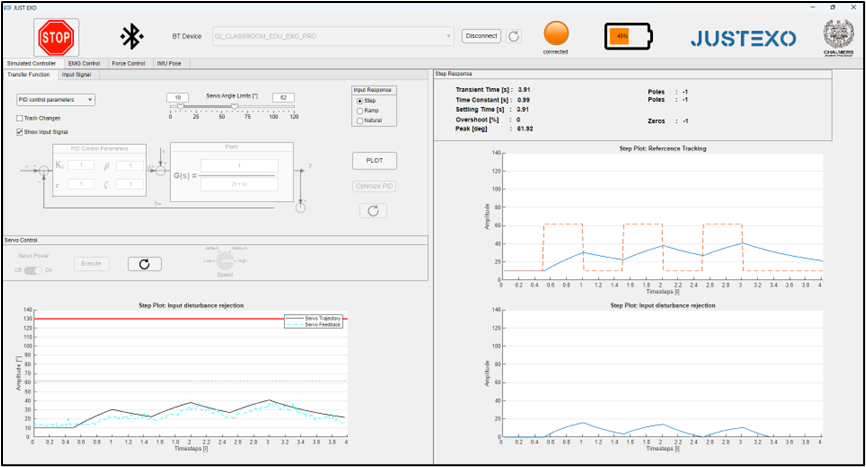
\includegraphics[width=0.7\linewidth]{img/fig_11}
	\caption{The GUI for the simulated PID control parameters.}
	\label{fig:fig11}
\end{figure}


There are three real-time measurement graphs available for monitoring system behavior. One graph tracks reference signals following (input (red) and output (blue)). The other two graphs are used to monitor input disturbance rejection. The graph in the right corner, shows the system's response to a disturbance signal. It measures how well the system can reject or minimize the effect of disturbances that deviate the system from its desired state. The other graph next to it, has a clear red line at the top of the graph. This line is the danger zone, and it is important that the signal does not pass this line. The graph also shows the servo trajectory (the calculated trajectory) in black, and the servo feedback (how the motor actually moves) in blue.

\newpage
\subsection{PI/PID setup}
The exoskeleton should be put on before starting this part.
1.	Choose the “Simulated controller” tab, and then the “transfer function” tab, which can be seen in \autoref{fig:fig12}.

\begin{figure}[H]
	\centering
	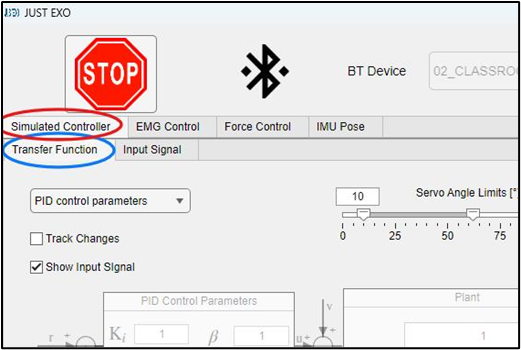
\includegraphics[width=0.7\linewidth]{img/fig_12}
	\caption{Choosing the simulated controller tab (red) and the transfer function tab (blue).}
	\label{fig:fig12}
\end{figure}


2.	Choose input response, see \autoref{fig:fig13}.
\begin{figure}[H]
	\centering
	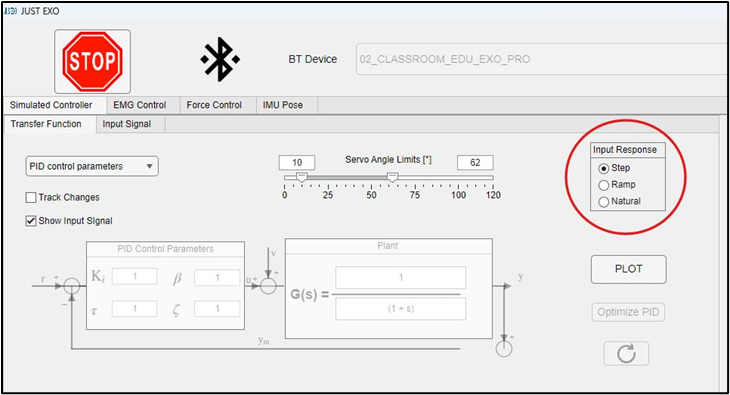
\includegraphics[width=0.7\linewidth]{img/fig_13}
	\caption{Choosing the input response.}
	\label{fig:fig13}
\end{figure}

3.	In the dropdown menu, choose which controller you want to work with. See \autoref{fig:fig14}.
\begin{figure}[H]
	\centering
	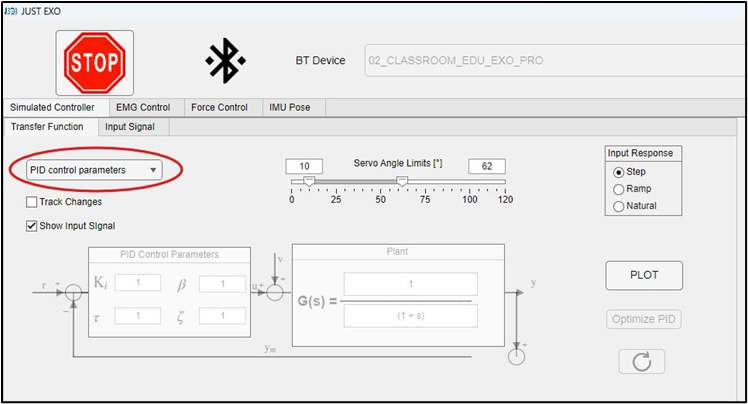
\includegraphics[width=0.7\linewidth]{img/fig_14}
	\caption{In the dropdown menu (red) choose controller.}
	\label{fig:fig14}
\end{figure}

4.	Choose parameters, see \autoref{fig:fig15}.
\begin{figure}[H]
	\centering
	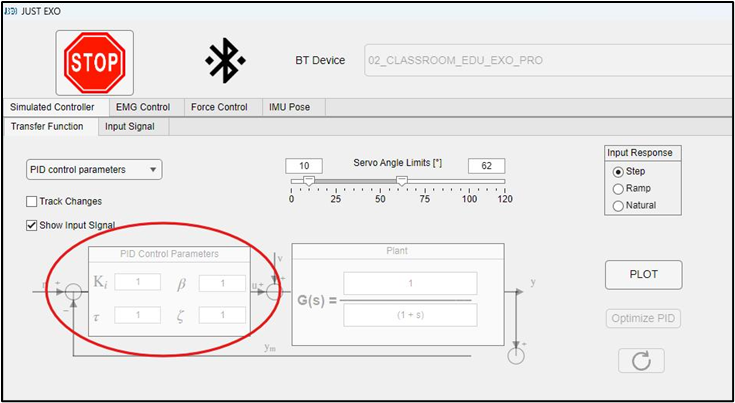
\includegraphics[width=0.7\linewidth]{img/fig_15}
	\caption{Change the different parameters.}
	\label{fig:fig15}
\end{figure}

5.	Click on the input signal tab, see \autoref{fig:fig16}.

\begin{figure}[H]
	\centering
	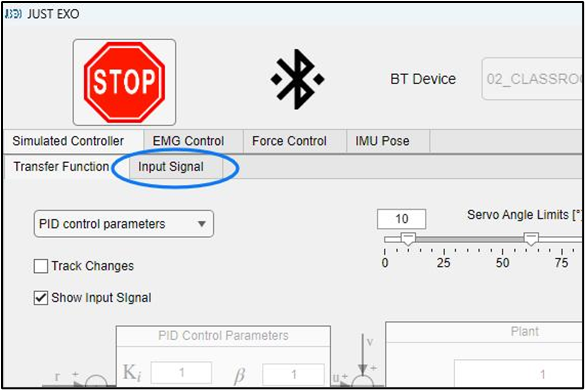
\includegraphics[width=0.7\linewidth]{img/fig_16}
	\caption{The input signal tab (blue).}
	\label{fig:fig16}
\end{figure}


6.	In this tab, you can modify the parameters for the input signal, such as the period and the number of repetitions, to suit your needs. See \autoref{fig:fig17}.
\begin{figure}[H]
	\centering
	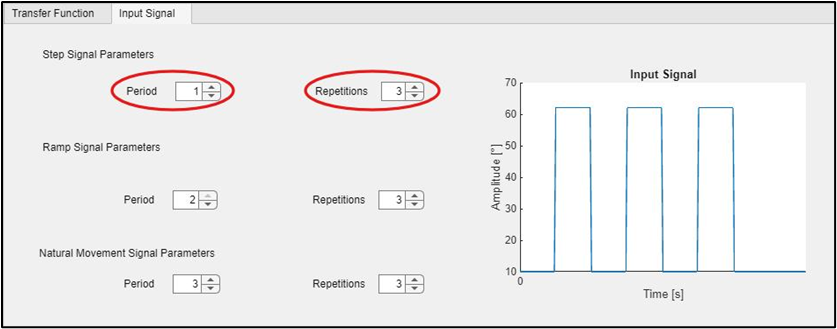
\includegraphics[width=0.7\linewidth]{img/fig_17}
	\caption{Choosing the period and repetitions}
	\label{fig:fig17}
\end{figure}


7.	When you have chosen the parameters for the input response, go back to the “Transfer Function” tab, and click on plot. You should now see three different plots. See \autoref{fig:fig18}
a.	If you get an error that says “The used system (TF) is crosses the Danger zone (0°).”, see page 18 for more information.
\begin{figure}[H]
	\centering
	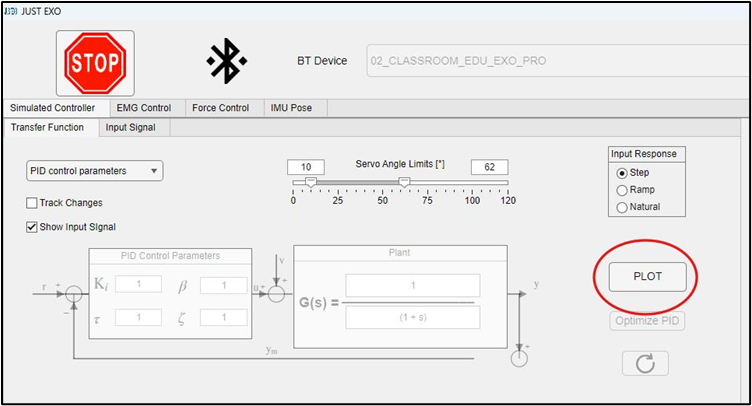
\includegraphics[width=0.7\linewidth]{img/fig_18}
	\caption{Click plot.}
	\label{fig:fig18}
\end{figure}




8.	Below the title Servo Control, click on server power (on), see figure 19. The Classroom Exo should move to the reference angle.

9.	Before clicking execute, you can change the speed. Click the knob-like button, and choose low, default, medium or high. See \autoref{fig:fig19}.
10.	Then click execute, see \autoref{fig:fig19}. The Classroom Exo should then start moving. (The button should turn magenta/purple/pink)
11.	If you click on the reset button next to the execute one, see \autoref{fig:fig19}, the Classroom Exo should return to the reference angle and you should be able to click execute again.
\begin{figure}[H]
	\centering
	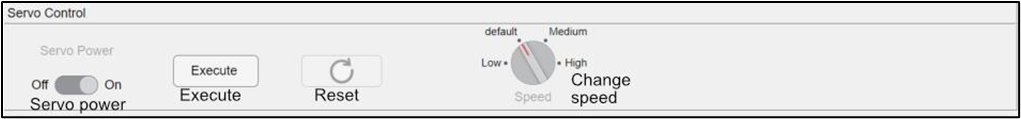
\includegraphics[width=1\linewidth]{img/fig_19}
	\caption{Layout for servo control.}
	\label{fig:fig19}
\end{figure}


\newpage
\section{Exercises}
This section outlines a series of exercises to be completed during the allotted lab time. These exercises are designed to deepen your understanding of how a simulated PI/PID control can be applied in combination with the Classroom Exo. The question exercises are meant to be discussed within a group. 

\subsection{Tasks and questions PI}
Below are a number of tasks and questions related to the PI controller. These tasks are designed to help you explore the behavior of the PI controller under different conditions and parameter settings.

\subsubsection{Trying out the PI controller}
These initial tasks will allow you to get comfortable with the simulation interface and begin exploring how altering different parameters influences the system's performance.
\paragraph{Task:}
\begin{enumerate}[]
	\item Choose the PI design parameters in the drop-down menu.
	\item Set $\omega_c$ = 2 and  $\phi_m$ = 45
	\item The click plot.
	\item When the graphs have appeared, turn on the servo power and then click execute. 
	\begin{enumerate}[]
		\item If you can’t click on execute, then restart the GUI, see more information on page 18.
	\end{enumerate}
\end{enumerate}

\paragraph{Questions}:
\begin{enumerate}[]
	\item What happens?
	\item Why does it lead to this result?
\end{enumerate}

\paragraph{Task: }
\begin{enumerate}[]
	\item Choose the PI control parameters in the drop-down menu.
	\item Set  Ki = 1.5 and Ti = 5.
	\item The click plot.
	\item When the graphs have appeared, turn on the servo power and then click execute. 
\end{enumerate}

\paragraph{Questions:}
\begin{enumerate}[]
	\item What happens?
	\item Why does it lead to this result?
\end{enumerate}



\subsubsection{Changing the input response} 
Choose another input response, and go to the Input Signal tab. Now, change the parameter values for Period and Repetition to observe how the input signal affects the system. You may choose any period and repetition, however the period needs to be an integer value. This task is designed to help you understand the impact of the input signal on the system’s response.
\paragraph{Task:}
\begin{enumerate}[]
	\item Choose the PI design parameter
	\item Set $\omega_c$ = 2 and $\phi_m$ = 45
	\item The click plot
	\item When the graphs have appeared, turn on the servo power and then click execute.
\end{enumerate}
\paragraph{Questions:}
\begin{enumerate}[]
	\item Is there any difference between this result, and the result from section 4.1.1?
	\begin{enumerate}
	\item Why is there a difference?
	\end{enumerate}
	\item How does the input response affect the control system?
	\item Do you notice any difference in system response between step, ramp and natural input signal?
\end{enumerate}

\newpage
\subsubsection{Working with the PI controller}
Below are a series of general questions related to the PI controller. These questions involve parameter adjustments of the upper crossover frequency and phase margin, and exploring optimized values. To solve these tasks, begin by selecting parameter values for Period and Repetition in the input signal tab.
\paragraph{Task:}
\begin{enumerate}[]
	\item Choose the PI design parameter in the drop-down menu.
	\item Increase crossover frequency $\omega_c$ while the phase margin $\phi_m$ remains the same. What do you observe?
	\item While still having a high crossover frequency $\omega_c$  increase the phase margin $\phi_m$. What do you observe?
	\item Test other lower values for $\omega_c$ and $\phi_m$.
\end{enumerate}
\paragraph{Questions:}
\begin{enumerate}[]
	\item How do the different parameter values affect the system’s behavior?
	\item These parameters are dependent on each other and affect the system's response. How does one choice affect the choice of another?
	\item What happens with the system response if you keep one of the parameters constant, and change only the other?
	\item How does the crossover frequency $\omega_c$ affect stability at low phase margins?
\end{enumerate}
\paragraph{Task:}
\begin{enumerate}[]
	\item Choose the PI control parameter in the drop-down menu.
	\item Set the integral component Ki close to zero (e.g. 0.2).
\end{enumerate}
\paragraph{Questions:}
\begin{enumerate}[]
	\item Can you see a steady state error?
	\item How does a low Ki affect the steady-state error and the system's stability?
	\item What happens if you set Ki to a high value? Why?
\end{enumerate}
\paragraph{Task:}
\begin{enumerate}[]
	\item Choose the PI control parameter in the drop-down menu.
	\item Try out some different values of Ki and Ti.
\end{enumerate}
\paragraph{Questions:}
\begin{enumerate}[]
	\item How does Ti  affect the control system? Keep Ki constant.
	\begin{enumerate}[]
	\item What would happen if Ti  had a low value? 
	\item What would happen if Ti  had a high value?
	\end{enumerate}
	\item How does Ki  affect the control system? Keep Ti  constant.
	\begin{enumerate}[]
	\item What would happen if Ki  had a low value? 
	\item What would happen if Ki  had a high value?
	\end{enumerate}
\end{enumerate}


\newpage
\subsection{Tasks and questions PID}
Below are several tasks and questions related to the PID controller. These tasks are designed to help you explore the behavior of the PID controller under different conditions and parameter settings
\subsubsection{Trying out the PID controller}
These initial tasks will allow you to get comfortable with the simulation interface and begin exploring how altering different parameters influences the system's performance.
\paragraph{Task:}
\begin{enumerate}[]
	\item Choose the PID design parameters in the drop-down menu.
	\item Set  $\omega_c$ = 3 , $\beta$ = 5 and $\phi_m$ = 65.What happens?
	\item Increase and decrease the crossover frequency $\omega_c$
	\item Increase and decrease the phase margin $\phi_m$
\end{enumerate}
\paragraph{Questions:}
\begin{enumerate}[]
	\item How do the crossover frequency and phase margin affect the system’s behavior?
	\item How do these parameters affect each other?
	\item What happens if you keep one of the parameters constant and change only the other one?
	\item How does the crossover frequency $\omega_c$ affect stability at low phase margins?
\end{enumerate}
\paragraph{Task:}
\begin{enumerate}[]
	\item Set $\beta$ to 1.
	\item Then set $\beta$ to 30.
\end{enumerate}
\paragraph{Questions:}
\begin{enumerate}[]
	\item What happens if you set $\beta$ to 1?
	\item What happens if $\beta$ is larger?
	\item What effect does the constant have on the controller?
\end{enumerate}
\paragraph{Task:}
\begin{enumerate}[]
	\item Choose the PID control parameters in the drop-down menu.
	\item Chose values for Ki, $\tau$, and $\beta$. For example, set Ki = 1, $\tau$ = 10 and $\beta$ = 12.
	\item Try different values for the damping factor $\zeta$.
\end{enumerate}
\paragraph{Questions:}
\begin{enumerate}[]
	\item What happens to the system’s behavior when the damping factor $\zeta$ increases?
	\item What effect does the damping factor $\zeta$ have on the system?
	\item How do the Ki, $\beta$, $\tau$, and $\zeta$ affect the control system’s performance?
\end{enumerate}
\paragraph{Task:}
\begin{enumerate}[]
	\item Now hold $\beta$ and $\zeta$ constant and set Ki close to zero.
	\item Experiment with different values for $\tau$
\end{enumerate}
\paragraph{Questions:}
\begin{enumerate}[]
	\item What happens if you set Ki to a high value?
	\item What effect does the integral component have on the system?
	\item How do these two parameters affect the time it takes for the system to reach a steady state?
	\item What effect does $\tau$ have on the system?
	\begin{enumerate}[]
		\item What would happen if $\tau$ was large?
	\end{enumerate}
\end{enumerate}

\subsubsection{Changing the input response }
Choose another input response, and go to the Input Signal tab. Now, change the parameter values for Period and Repetition to observe how the input signal affects the system. This task is designed to help you understand the impact of the input signal on the system’s response.

\paragraph{Task:}
\begin{enumerate}[]
	\item Choose the PID design parameter. 
	\item Set $\omega_c$ = 3 , $\beta$ = 5 and $\phi_m$ = 65.
	\item Then click plot.
	\item When the graphs have appeared, turn on the servo power and then click execute.
\end{enumerate}
\paragraph{Questions:}
\begin{enumerate}[]
	\item Is there any difference between this result, and the result from section 4.2.1? Why or why not?
	\item How does the input response affect the control system?
	\item How does the system handle a step, ramp, and natural input?
\end{enumerate}


\newpage
\section{Discussion}
For the best learning experience, feel free to discuss the results your group obtained from each step between groups to gain understanding and new perspectives.
\begin{enumerate}
	\item What do the graphs tell you about the system’s behavior? 
	\begin{enumerate}[]
		\item What conclusions can you draw regarding parameter choices from these graphs? What can be deduced?
	\end{enumerate}
	\item Compare the different controllers to each other. Which one works best for the Classroom Exo? 
	\begin{enumerate}
		\item Are there cases where the PI controller would work better than the PID, and vice versa?
	\end{enumerate}
	\item How do PI and PID controllers influence user safety when applied in biomedical devices like exoskeletons? Consider factors such as system stability, responsiveness, and the potential for overshooting or oscillations.
	\begin{enumerate}[]
		\item How could improper calibration or tuning of these controllers lead to risks for the user, such as joint misalignment or muscle strain?
		\item What are some preventative measures that could be taken to minimize these risks when implementing control systems in devices that support or augment human movement?
	\end{enumerate}
\end{enumerate}



\section{Typical errors and Troubleshooting}
In this section, we present typical errors and issues encountered during testing of the Classroom Exo. 
\begin{enumerate}
	\item If you get an error message that says “The used system (TF) is crosses the Danger zone (0°). Please try another system or change the minimum servo angle limits.”, then you can  increase the input server angle limit or change control parameters and plot again. 
	\item If you get this error message it is because you can't choose a period that is not a whole number. 
	\item For design parameters, after plotting you cannot change the parameter values, this is a bug. Switch to another control in the drop-down menu. And switch back to the design parameter of your choice and you should be able to choose parameter values.
	\item If you can’t click on execute after you clicked plot (the execute button is not visible), then you need to restart the GUI and connect to the Classroom Exo again.
\end{enumerate}

\begin{tcolorbox}[colback=green!5!white,colframe=green!75!black,title=Hint]
	You can find a more comprehensive Troubleshooting documentation in the Manual on our GitHub!
\end{tcolorbox}
\vspace{0.5cm}


	




